\let\negmedspace\undefined
\let\negthickspace\undefined
\documentclass[journal]{IEEEtran}
\usepackage[a5paper, margin=10mm, onecolumn]{geometry}
%\usepackage{lmodern} % Ensure lmodern is loaded for pdflatex
\usepackage{tfrupee} % Include tfrupee package

\setlength{\headheight}{1cm} % Set the height of the header box
\setlength{\headsep}{0mm} % Set the distance between the header box and the top of the text

\usepackage{gvv-book}
\usepackage{gvv}
\usepackage{cite}
\usepackage{amsmath,amssymb,amsfonts,amsthm}
\usepackage{algorithmic}
\usepackage{graphicx}
\usepackage{textcomp}
\usepackage{xcolor}
\usepackage{txfonts}
\usepackage{listings}
\usepackage{enumitem}
\usepackage{mathtools}
\usepackage{gensymb}
\usepackage{comment}
\usepackage[breaklinks=true]{hyperref}
\usepackage{tkz-euclide} 
\usepackage{listings}
% \usepackage{gvv}                                        
\def\inputGnumericTable{}                                 
\usepackage[latin1]{inputenc}                                
\usepackage{color}                                            
\usepackage{array}                                            
\usepackage{longtable}                                       
\usepackage{calc}                                             
\usepackage{multirow}                                         
\usepackage{hhline}                                           
\usepackage{ifthen}                                           
\usepackage{lscape}
\begin{document}

\bibliographystyle{IEEEtran}
\vspace{3cm}

\title{1.9.22}
\author{EE25BTECH11033 - Kavin}
% \maketitle
% \newpage
% \bigskip
{\let\newpage\relax\maketitle}

\renewcommand{\thefigure}{\theenumi}
\renewcommand{\thetable}{\theenumi}
\setlength{\intextsep}{10pt} % Space between text and floats
\textbf{Question}:\\
Find the value of $y$ for which the distance between the points $\vec{P}(2,-3)$ and $\vec{Q}(10,y)$ is $10$ units.\\
\bigskip

\textbf{Solution}:\\
Given the points,
\begin{align}
    \vec{P}=\begin{myvec}{2\\-3}\end{myvec}\ \ 
    \vec{Q}=\begin{myvec}{10\\y}\end{myvec}
\end{align}
The distance between the points \vec{P} and \vec{Q} is given as,
\begin{align}
d = \norm{\vec{P}-\vec{Q}} = 10\\
\end{align}
We know that, the length of a vector is defined as
\begin{align}
\label{eq:side-length}
	\norm{\vec{P}-\vec{Q}} \triangleq \sqrt{(\vec{P}-\vec{Q})^{\top}(\vec{P}-\vec{Q})}
		\\
(\vec{P}-\vec{Q})^\top (\vec{P}-\vec{Q}) = \norm{\vec{P}-\vec{Q}}^2\\
(\vec{P}-\vec{Q})^\top (\vec{P}-\vec{Q}) = 10^2\\
\end{align}
\begin{align}
\because
		\vec{P} - \vec{Q} = \myvec{2\\-3} - \myvec{10\\y} &= \myvec{-8\\-3-y},\\
        \implies\myvec{-8\\-3-y}^\top\myvec{-8\\-3-y} &= 10^2\\
        \implies\myvec{-8 & -3-y}\myvec{-8\\-3-y} &= 100\\
        \implies8^2 + (3+y)^2 = 100\\
        \implies(3+y)^2=36\\
        \implies3+y=\pm6\\
        \implies y=3, -9
\end{align}
Therefore the points $\brak{10,3}$ and $\brak{10,-9}$ are at a distance of $10$ units from the point \vec{P}.
\bigskip

See Fig. 0 ,
\newpage
\begin{figure}[H]
\begin{center}
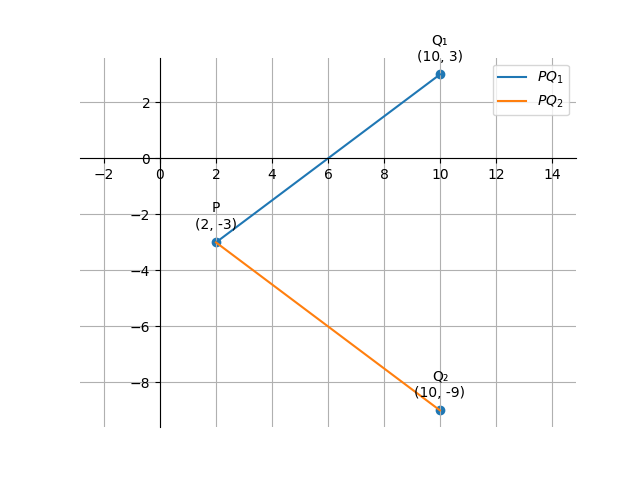
\includegraphics[width=0.8\columnwidth]{figs/fig.png}
\end{center}
\caption{}
\label{fig:Fig1}
\end{figure}

\end{document}